\documentclass[aspectratio=169,10pt]{beamer}

\usetheme{default}
\setbeamertemplate{navigation symbols}{}
\setbeamertemplate{footline}{%
  \hfill\usebeamerfont{page number in head/foot}\insertframenumber/\inserttotalframenumber\hspace{1.2em}\vspace{0.8em}
}
\setbeamertemplate{itemize item}{\raise0.2ex\hbox{\scriptsize$\blacktriangleright$}}
\setbeamertemplate{itemize subitem}{\raise0.2ex\hbox{\scriptsize$\triangleright$}}

\usepackage[T1]{fontenc}
\usepackage{lmodern}
\usepackage{amsmath,amssymb,booktabs,array,multirow}
\usepackage{graphicx}
\usepackage{tikz}
\usepackage[numbers,sort&compress]{natbib}
\providecommand{\doi}[1]{}
\usetikzlibrary{arrows.meta,positioning,calc}

\definecolor{ink}{RGB}{22,31,45}
\definecolor{slate}{RGB}{48,61,78}
\definecolor{muted}{RGB}{94,105,118}
\definecolor{rulegray}{RGB}{190,196,204}
\definecolor{deepblue}{RGB}{18,52,86}
\definecolor{wine}{RGB}{124,36,45}
\definecolor{forest}{RGB}{34,93,73}
\definecolor{paper}{RGB}{250,250,248}

\setbeamercolor{normal text}{fg=ink,bg=paper}
\setbeamercolor{frametitle}{fg=deepblue,bg=paper}
\setbeamercolor{title}{fg=deepblue}
\setbeamercolor{subtitle}{fg=slate}
\setbeamercolor{structure}{fg=deepblue}
\setbeamercolor{alerted text}{fg=wine}
\setbeamerfont{title}{series=\bfseries,size=\Large}
\setbeamerfont{frametitle}{series=\bfseries,size=\large}
\setbeamerfont{author}{size=\normalsize}
\setbeamerfont{date}{size=\small}
\setbeamerfont{jointwork}{size=\scriptsize}

\setlength{\parskip}{0.25em}
\renewcommand{\arraystretch}{1.18}

\newcommand{\E}{\mathbb{E}}
\newcommand{\Pbb}{\mathbb{P}}
\newcommand{\one}{\mathbf{1}}
\newcommand{\surv}{p_{\mathrm{surv}}}
\newcommand{\liq}{p_{\mathrm{liq}}}
\newcommand{\hf}{H}
\newcommand{\diff}{\mathrm{d}}

\title[Evaluating leveraged DeFi long--short positions]{Evaluating Leveraged DeFi Long--Short Positions under Jump Risk: Killed Moments, Liquidation Recovery and the Limits of Optimal Sizing}
\author{Francis Liu}
\institute{Working paper}
\date{\today}

\begin{document}

% ------------------------------------------------------------
\begin{frame}
  \vspace{1.0em}
  {\usebeamerfont{title}\usebeamercolor[fg]{title}\inserttitle\par}
  \vspace{1.2em}
  {\usebeamerfont{author}\insertauthor\par}
  \vspace{0.7em}
  {\usebeamerfont{jointwork}
    Joint work with Professor Daniel Pele, Department of Statistics and Econometrics,\\
    Bucharest University of Economic Studies\\
    Theodor Ginavar, PhD Candidate, MSCA Digital Finance\par}
  {\usebeamerfont{date}\insertinstitute\hspace{0.6em}|\hspace{0.6em}\insertdate\par}
  \vfill
  \begin{center}
    
\begin{tikzpicture}
      \draw[deepblue,very thick] (0,0) -- (10.8,0);
      \draw[wine,thick] (0,-0.12) -- (2.4,-0.12);
    \end{tikzpicture}
  \end{center}
  \vspace{0.8em}
  \large DeFi long--short sizing under liquidation and jump risk
\end{frame}

% ------------------------------------------------------------
\begin{frame}{DeFi Lending Platforms}
  \small
  Aave / Compound: pooled lending
  \vspace{0.4em}

  \begin{itemize}
    \item \textbf{Mechanism} lenders supply pool assets; borrowers draw pooled liquidity
    \item \textbf{Accounting} no bilateral lender; protocol-level collateral and debt balances
    \item \textbf{Interest accrual} variable supply/borrow APRs; utilization-driven index growth
    \item \textbf{No fixed tenor} open-ended loans; no maturity date; no term structure contract
  \end{itemize}

  \vspace{0.25em}
  \textbf{Overcollateralization}
  \begin{itemize}
    \item Pseudonymous parties; no credit underwriting; no legal margin call
    \item Solvency and obligation enforcement entirely collateral-based
    \item No-arbitrage discipline through collateral constraint
    \item \textbf{Liquidator role} repay unsolvent debt; seize collateral bonus; restore pool solvency
  \end{itemize}

\end{frame}

% ------------------------------------------------------------
\begin{frame}{Health Factor and Boundary}
  \small
  {\bf{Key mechanism variables}}
  \vspace{0.35em}

  State variables:
  \[
    V_{1,t}:=n_1S_{1,t}\quad\text{collateral value},
    \qquad
    V_{2,t}:=n_2S_{2,t}\quad\text{borrow/debt value}
  \]
  \vspace{0.25em}

  Loan-to-value* and liquidation threshold:
  \[
    \mathrm{LTV}_t:=\frac{V_{2,t}}{V_{1,t}},
    \qquad
    b=\mathrm{threshold\ LTV}
  \]
  Aave origination LTV $<$ threshold LTV $b$; initial buffer by design
  \vspace{0.25em}

  Health factor:
  \[
    H_t:=\frac{b\,V_{1,t}}{V_{2,t}}
    =
    \frac{b}{\mathrm{LTV}_t}
  \]
  \vspace{0.25em}

  Liquidation triggering condition:
  \[
    H_t<1
    \quad\Longleftrightarrow\quad
    V_{2,t}>b\,V_{1,t}
  \]

  {\scriptsize * Remark: for now, ignore origination-LTV / threshold-LTV gap}
  \vspace{0.2em}
\end{frame}

% ------------------------------------------------------------
\begin{frame}{Constructing the Long--Short Position}
  \begin{center}
    \begin{tabular}{@{}p{0.15\linewidth}p{0.45\linewidth}p{0.30\linewidth}@{}}
      \toprule
      Step & Protocol action & Economic exposure \\
      \midrule
      0 & Initial capital injection: \$1-worth BTC & External capital only \\
      1 & Supply BTC collateral to Aave & Long BTC collateral \\
      2 & Borrow \$0.8-worth ETH & Short ETH liability \\
      3 & Sell ETH into \$0.8-worth BTC & Self-financing conversion \\
      4 & Re-supply BTC as collateral & Total BTC collateral: \$1.8 \\
      \midrule
      Result & Collateralized debt position & Leveraged long BTC, short ETH \\
      \bottomrule
    \end{tabular}
  \end{center}
  \vspace{0.55em}
  Resulting normalized position:
  \begin{itemize}
    \item External capital: \$1; no additional capital after step 0
    \item BTC collateral: \$1.8; ETH debt: \$0.8
    \item $b=0.8$; $H_0=0.8\times1.8/0.8=1.8$
    \item Leveraged BTC exposure; short ETH exposure
  \end{itemize}
\end{frame}

% ------------------------------------------------------------
\begin{frame}{Looping the Position}
  \small
  Repeat steps 1--4; zero transaction cost and slippage
  \vspace{0.35em}

  Round-$m$ additional collateral:
  \[
    1,\quad b,\quad b^2,\quad \ldots,\quad b^m
  \]
  Total BTC collateral after $m$ loops:
  \[
    V_1^{(m)}
    =
    1+b+\cdots+b^m
    =
    \frac{1-b^{m+1}}{1-b}
  \]
  ETH debt:
  \[
    V_2^{(m)}
    =
    b+b^2+\cdots+b^{m+1}
    =
    b\,V_1^{(m)}
  \]
  Infinite-loop limit:
  \[
    V_1^{(\infty)}=\frac{1}{1-b},
    \qquad
    V_2^{(\infty)}=\frac{b}{1-b}
  \]
  Example $b=0.8$:
  \[
    V_1^{(\infty)}=5,
    \qquad
    V_2^{(\infty)}=4,
    \qquad
    H_0^{(\infty)}=\frac{bV_1^{(\infty)}}{V_2^{(\infty)}}=1
  \]
  Extreme leverage: any adverse move $\rightarrow$ liquidation; favorable move $\rightarrow$ amplified gain
\end{frame}

% ------------------------------------------------------------
\begin{frame}{Unwinding and Taking Profit}
  \small
  Favorable scenario: BTC $+10\%$; ETH $-16.7\%$
  \[
    H_t=\frac{0.80\,V_{1,t}}{V_{2,t}},
    \qquad
    \text{equity}=V_{1,t}-V_{2,t}
  \]
  \vspace{0.15em}
  \begin{center}
    \begin{tabular}{@{}p{0.17\linewidth}r r c r p{0.20\linewidth}@{}}
      \toprule
      Scenario & BTC collat. & ETH debt & $H$ & Equity & Action \\
      \midrule
      Entry & \$1.80 & \$0.80 & $1.80$ & \$1.00 & Hold \\
      Favorable move & \$1.98 & \$0.667 & $2.38$ & \$1.313 & Voluntary unwind \\
      \bottomrule
    \end{tabular}
  \end{center}
  \vspace{0.5em}
  Outcome:
  \[
    \text{gain}=1.313-1.000=0.313
  \]
  Voluntary unwind; solvent position; profit realization
\end{frame}

% ------------------------------------------------------------
\begin{frame}{Aave Liquidation and Immediate Risk}
  \small
  Adverse scenario: BTC $-25\%$; ETH $+40\%$
  \[
    H_t=\frac{bV_{1,t}}{V_{2,t}}
    =
    \frac{0.80\,V_{1,t}}{V_{2,t}},
    \qquad
    H_t\leq1
    \Longleftrightarrow
    \frac{V_{2,t}}{V_{1,t}}\geq0.80
  \]
  \vspace{0.15em}
  \begin{center}
    \begin{tabular}{@{}p{0.17\linewidth}r r c r p{0.20\linewidth}@{}}
      \toprule
      Scenario & BTC collat. & ETH debt & $H$ & Equity & Outcome \\
      \midrule
      Entry & \$1.80 & \$0.80 & $1.80$ & \$1.00 & Safe \\
      Adverse move & \$1.35 & \$1.12 & $0.96$ & \$0.23 & Liquidatable \\
      \bottomrule
    \end{tabular}
  \end{center}
  \vspace{0.35em}
  Outcome:
  \[
    H_t<1
    \quad\Rightarrow\quad
    \text{keeper liquidation; collateral seized at bonus}
  \]
  Recovery drivers: shock severity; market sentiment/liquidity; liquidator inventory willingness; gas fees
  \vspace{0.2em}

  Modeling convention: detailed recovery omitted; $\Pi_T=0$ whenever $\tau\le T$
\end{frame}

% ------------------------------------------------------------
\begin{frame}{Payoff Function from the Trade}
  \small
  Holdings: $n_1$ units of collateral asset $S_1$; debt: $n_2$ units of borrowed asset $S_2$
  \vspace{0.3em}

  Surviving-path terminal wealth:
  \[
    \Pi_T:=(n_1S_{1,T}-n_2S_{2,T})\,\one_{\{\tau>T\}}
  \]
  Running BTC/ETH example:
  \[
    S_1=\mathrm{BTC},\qquad S_2=\mathrm{ETH},
    \qquad n_1S_{1,0}=1.80,\qquad n_2S_{2,0}=0.80
  \]
  Therefore:
  \[
    \Pi_T=
    \left(
      1.80\,\frac{S_{1,T}}{S_{1,0}}
      -
      0.80\,\frac{S_{2,T}}{S_{2,0}}
    \right)\one_{\{\tau>T\}}
  \]
  Survival indicator: $\tau\le T \Rightarrow \Pi_T=0$
  \vspace{0.25em}

  Initial net book value normalized to one unit of account; moments stated directly in $\Pi_T$
\end{frame}

% ------------------------------------------------------------
\begin{frame}{Why Payoff Moments Are Hard}
  \small
  Target statistics:
  \[
    \E[\Pi_T],\qquad
    \mathrm{Var}(\Pi_T),\qquad
    \E[\Pi_T^k],\quad k\ge1
  \]
  Killed payoff:
  \[
    \Pi_T^k
    =
    (n_1S_{1,T}-n_2S_{2,T})^k
    \one_{\{\tau>T\}}
  \]
  Terminal payoff state:
  \[
    (S_{1,T},S_{2,T})
  \]
  Pathwise killing process:
  \[
    \tau>T
    \quad\Longleftrightarrow\quad
    H_s\ge1\ \text{ for all }s\le T,
    \qquad
    H_s=\frac{b\,n_1S_{1,s}}{n_2S_{2,s}}
  \]
  Direct moment:
  \[
    \E_\Pbb[\Pi_T^k]
    =
    \E_\Pbb\!\left[(n_1S_{1,T}-n_2S_{2,T})^k\one_{\{\tau>T\}}\right]
  \]
  Difficulty: terminal bivariate payoff + pathwise barrier
  \vspace{0.25em}

  Generic numerical routes:
  \begin{itemize}
    \item Monte Carlo; barrier monitoring / possible 2D Brownian-bridge refinement
    \item Numerical PDE/PIDE; two terminal state variables plus killing boundary
  \end{itemize}
\end{frame}

% ------------------------------------------------------------
\begin{frame}{Literature Positioning}
  \small
  Intersection:
  \[
    \text{DeFi liquidation}
    \quad+\quad
    \text{first-passage methods for jump diffusions}
  \]
  \vspace{0.35em}

  \begin{itemize}
    \item \textbf{DeFi liquidation} Qin et al.~\cite{Qin2021}; Heimbach--Huang~\cite{HeimbachHuang2024}
    \item Incentive structure; leverage amplification; liquidation cascades
    \item Empirical focus; no ex-ante sizing rule
  \end{itemize}
  \vspace{0.25em}

  \begin{itemize}
    \item \textbf{First passage under jumps} Kou--Wang~\cite{KouWang2003}; Sepp~\cite{Sepp2004}
    \item Double-exponential jumps; Laplace transforms; finite algebraic systems
    \item Classical object: single-asset barrier option
  \end{itemize}
  \vspace{0.25em}

  Gap:
  \[
    \text{barrier-killed long--short ratio}
    \quad\neq\quad
    \text{single-asset barrier option}
  \]
  Bridge: change of measure $\rightarrow$ one-dimensional killed expectation
\end{frame}

% ------------------------------------------------------------
\begin{frame}{Price Process}
  \small
  Jump motivation: crypto gaps; flash crashes; barrier crossed before rebalance
  \hfill Kou model~\cite{Kou2002}
  \vspace{0.25em}

  Price dynamics, $i=1,2$:
  \[
    S_{i,t}=S_{i,0}e^{X_{i,t}},
    \qquad
    dX_{i,t}
    =
    \mu_i^X\,dt+\sigma_i\,dB_{i,t}
    +d\!\left(\sum_{n=1}^{N_{i,t}}J_i^{(n)}\right)
  \]
  Brownian correlation:
  \[
    d\langle B_1,B_2\rangle_t=\rho\,dt,
  \]
  Poisson intensity: $\lambda_i$
  \vspace{0.2em}

  Kou double-exponential jump density:
  \[
    f_i(j)
    =
    \frac{p_i}{\eta_{i,+}}e^{-j/\eta_{i,+}}\one_{\{j>0\}}
    +
    \frac{1-p_i}{\eta_{i,-}}e^{j/\eta_{i,-}}\one_{\{j<0\}}
  \]
  Drift normalization: $\E_\P[S_{i,t}/S_{i,0}]=e^{\mu_i t}$
  \[
    \mu_i^X=\mu_i-\frac12\sigma_i^2-\lambda_i\chi_i,
    \qquad
    \chi_i=\E[e^{J_i}-1]
    =
    \frac{p_i}{1-\eta_{i,+}}+\frac{1-p_i}{1+\eta_{i,-}}-1
  \]
  Constant supply/borrow rates absorbed into drift; dynamic rate modeling outside scope
\end{frame}

% ------------------------------------------------------------
\begin{frame}{Semi-Analytic Architecture}
  \small
  \begin{center}
    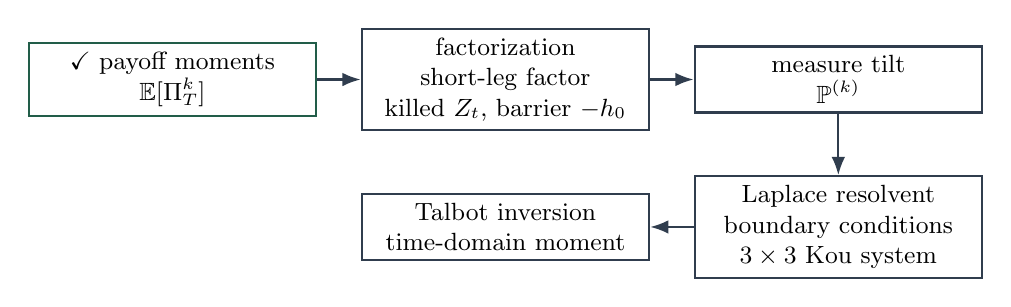
\begin{tikzpicture}[
      stage/.style={draw=slate,thick,minimum width=3.65cm,minimum height=0.82cm,align=center,font=\small},
      done/.style={draw=forest,thick,minimum width=3.65cm,minimum height=0.82cm,align=center,font=\small},
      arr/.style={-Latex,thick,slate}
    ]
      \node[done] (a) {$\checkmark$ payoff moments\\$\E[\Pi_T^k]$};
      \node[stage,right=0.55cm of a] (b) {factorization\\short-leg factor\\killed $Z_t$, barrier $-h_0$};
      \node[stage,right=0.55cm of b] (c) {measure tilt\\$\Pbb^{(k)}$};
      \node[stage,below=0.78cm of c] (d) {Laplace resolvent\\boundary conditions\\$3\times3$ Kou system};
      \node[stage,left=0.55cm of d] (e) {Talbot inversion\\time-domain moment};
      \draw[arr] (a) -- (b);
      \draw[arr] (b) -- (c);
      \draw[arr] (c) -- (d);
      \draw[arr] (d) -- (e);
    \end{tikzpicture}
  \end{center}
  \vspace{0.45em}
  Covered: payoff function + need for moments
  \vspace{0.25em}

  Next: factorization and measure change $\rightarrow$ one-dimensional killed expectation
  \[
    k\,\eta_{2,+}<1
    \quad\text{moment-admissibility condition}
  \]
\end{frame}

% ------------------------------------------------------------
\begin{frame}{Factorization: From Two Assets to One Barrier}
  \small
  Motivation: separate terminal short-leg factor; isolate killed ratio problem
  \vspace{0.25em}

  Bivariate payoff; scalar liquidation state:
  \[
    Z_t=X_{1,t}-X_{2,t}
  \]
  Initial log health factor:
  \[
    h_0:=\log H_0
  \]
  Factorization using $H_T=e^{h_0+Z_T}$:
  \[
    \Pi_T
    =
    \frac{n_2}{b}\,S_{2,0}e^{X_{2,T}}
    (e^{h_0+Z_T}-b)\,\one_{\{\tau>T\}}
  \]
  One-dimensional payoff kernel:
  \[
    g_k(z;h_0):=(e^{h_0+z}-b)^k,
  \]
  Integer moments:
  \[
  \begin{aligned}
    \Pi_T^k
    &=
    \underbrace{
      \Big(\frac{n_2}{b}\Big)^kS_{2,0}^k e^{kX_{2,T}}
    }_{\mathcal F_T^{S_2}\text{ part}}
    \underbrace{
      g_k(Z_T;h_0)\,\one_{\{\tau>T\}}
    }_{\mathcal F_T^{Z}\text{ killed-ratio part}}
  \end{aligned}
  \]
  Measure change: absorb $\mathcal F_T^{S_2}$ factor; retain killed expectation under $Z$
  \vspace{0.3em}

  Barrier-option analogue: scalar state $Z$, barrier $-h_0$
\end{frame}

% ------------------------------------------------------------
\begin{frame}{Measure Change}
  \scriptsize
  Start from factorized moment:
  \[
    \E_\Pbb[\Pi_T^k]
    =
    \Big(\frac{n_2}{b}\Big)^kS_{2,0}^k\,
    \E_\Pbb\!\left[
      e^{kX_{2,T}}g_k(Z_T;h_0)\one_{\{\tau>T\}}
    \right]
  \]
  Exponential tilt:
  \[
    \left.\frac{d\Pbb^{(k)}}{d\Pbb}\right|_{\mathcal F_T}
    =
    \frac{e^{kX_{2,T}}}{\E[e^{kX_{2,T}}]}
  \]
  Heuristic reminder, with $Y=g_k(Z_T;h_0)\one_{\{\tau>T\}}$:
  \[
  \begin{aligned}
    \E_{\Pbb^{(k)}}[Y]
    &=
    \int Y\,d\Pbb^{(k)}
    =
    \int Y\,\frac{d\Pbb^{(k)}}{d\Pbb}\,d\Pbb\\
    &=
    \E_\Pbb\!\left[
      Y\,\frac{e^{kX_{2,T}}}{\E_\Pbb[e^{kX_{2,T}}]}
    \right]
    &=
    \frac{\E_\Pbb[e^{kX_{2,T}}Y]}{\E_\Pbb[e^{kX_{2,T}}]}
    \quad\Longrightarrow\quad
    \E_\Pbb[e^{kX_{2,T}}Y]
    =
    \E_\Pbb[e^{kX_{2,T}}]\E_{\Pbb^{(k)}}[Y]
  \end{aligned}
  \]
  {\scriptsize Remark: Radon--Nikodym theorem / change-of-measure identity}
  \vspace{0.15em}

  Reduced moment:
  \[
    \E[\Pi_T^k]
    =
    \Big(\frac{n_2}{b}\Big)^kS_{2,0}^k
    \E[e^{kX_{2,T}}]\,
    \E^{(k)}\!\left[
      g_k(Z_T;h_0)\one_{\{\tau>T\}}
    \right]
  \]
  Bivariate payoff moment $\rightarrow$ killed expectation of the ratio process
\end{frame}

% ------------------------------------------------------------
\begin{frame}{Tilted Ratio Process}
  \small
  Remaining object:
  \[
    \E^{(k)}\!\left[
      g_k(Z_T;h_0)\one_{\{\tau>T\}}
    \right]
  \]
  Question:
  \[
    Z_t=X_{1,t}-X_{2,t}
    \quad\text{under}\quad \Pbb^{(k)}
  \]
  Under $\Pbb^{(k)}$: $Z$ remains a L\'evy process

  L\'evy--Khintchine exponent of $Z$ under $\Pbb^{(k)}$:
  \[
    \psi_Z^{(k)}(s)
    =
    \mu_Z^{(k)}s+\frac12\sigma_Z^2s^2
    +\lambda_1\big(M_1(s)-1\big)
    +\lambda_2\big(M_2(k-s)-M_2(k)\big)
  \]
  with
  \[
    M_i(s)=
    \frac{p_i}{1-s\eta_{i,+}}
    +
    \frac{1-p_i}{1+s\eta_{i,-}},
    \qquad
    \sigma_Z^2=\sigma_1^2+\sigma_2^2-2\rho\sigma_1\sigma_2
  \]
  $\mathcal L^{(k)}$: infinitesimal generator of $Z$ under $\Pbb^{(k)}$, the generator eigenrelation:
  \[
    \mathcal L^{(k)}e^{sz}=\psi_Z^{(k)}(s)e^{sz}
  \]
\end{frame}

% ------------------------------------------------------------
\begin{frame}{Killed Moment PIDE}
  \small
  Target function:
  \[
    U(t,z)
    :=
    \E_z^{(k)}\!\left[
      g_k(Z_t;h_0)\one_{\{\tau(h_0)>t\}}
    \right],
    \qquad z>-h_0
  \]
  \vspace{0.2em}

  Backward Kolmogorov PIDE for the killed process:
  \[
    \partial_t U(t,z)=\mathcal L^{(k)}U(t,z),
    \qquad z>-h_0
  \]
  Initial and absorbing boundary:
  \[
    U(0,z)=g_k(z;h_0),
    \qquad
    U(t,z)=0\quad\text{for }z\le -h_0
  \]
  \vspace{0.2em}
  
  One time variable; one state variable $z$ for the ratio process $Z$

\end{frame}

% ------------------------------------------------------------
\begin{frame}{Laplace Transform Trick}
  \small
  Time-domain PIDE:
  \[
    \partial_t U(t,z)=\mathcal L^{(k)}U(t,z),
    \qquad
    U(0,z)=g_k(z;h_0)
  \]
  Laplace transform in time:
  \[
    \widehat U(q,z)=\int_0^\infty e^{-qt}U(t,z)\,dt,
    \qquad q>0
  \]
  Laplace-domain resolvent:
  \[
    (q-\mathcal L^{(k)})\widehat U(q,z)=g_k(z;h_0),
    \qquad z>-h_0
  \]
  Sepp~\cite{Sepp2004} idea:

  Laplace transform $+$ double-exponential jumps $\rightarrow$ finite algebraic system
  \vspace{0.25em}

  Here:
  \[
    \psi_Z^{(k)}(\gamma)=q
    \quad\Longrightarrow\quad
    \text{degree-six characteristic equation}
  \]
  Three admissible roots $+$ three boundary conditions $\rightarrow 3\times3$ system
\end{frame}

% ------------------------------------------------------------
\begin{frame}{Resolvent Solution Form}
  \small
  Resolvent decomposition:
  \[
    \widehat U(q,z;h_0)
    =
    \widehat U_{\mathrm{part}}(q,z;h_0)
    +
    \widehat U_{\mathrm{hom}}(q,z;h_0)
  \]
  Particular solution:
  \[
    \widehat U_{\mathrm{part}}(q,z;h_0)
    =
    \sum_{j=0}^{k}
    \frac{c_{k,j}(h_0)}{q-\psi_Z^{(k)}(j)}e^{jz}
  \]
  Homogeneous solution:
  \[
    \widehat U_{\mathrm{hom}}(q,z;h_0)
    =
    \sum_{m=1}^{3}
    B_m^{(k)}(q;h_0)e^{\gamma_{m+3}(q)(z+h_0)}
  \]
  Boundary coefficients:
  \[
    \underbrace{\mathbf M_{\mathrm{bar}}^{(k)}(q)}_{3\times3}
    \underbrace{\mathbf B^{(k)}}_{3\times1}
    =
    -\underbrace{\mathbf b^{(k)}}_{3\times1}
  \]
  PIDE solve $\rightarrow$ summation of exponentials $+$ one $3\times3$ linear system
\end{frame}

% ------------------------------------------------------------
\begin{frame}{Benchmark: Drift Kept Outside the Fit}
  \small
  ECF on $840$ four-hour WBTC/WETH returns (Aave v3, 2026-03-17 to 08-04): $\sigma_i,\lambda_i,p_i,\eta_{i,\pm},\rho$
  \vspace{0.3em}

  \textbf{Drift is not fitted}
  \begin{itemize}
    \item Drift precision depends only on calendar length, not on sampling frequency
    \item A free drift in the ECF phase on de-meaned returns $=$ normalizer, not forecast ($\mu_1-\mu_2=-0.86$, wrong sign)
    \item Benchmark: window's sample drift incl.\ Aave rates, $\mu_1=-0.314$, $\mu_2=-0.417$
    \item Spread drift $\nu=\mu_1-\mu_2=+0.103$/yr ($+0.128$ price, $-0.025$ net carry)
  \end{itemize}
  \vspace{0.3em}
  \textbf{Any stated view can be substituted} --- the map is exact given its inputs
\end{frame}

% ------------------------------------------------------------
\begin{frame}{Validation Against Monte Carlo}
  \scriptsize
  \begin{columns}[T]
    \begin{column}{0.56\linewidth}
      \begin{tabular}{cc cc cc}
      \toprule
      $h_0$ & $H_0$ & $\surv^{\mathrm{Lap}}$ & $\surv^{\mathrm{MC}}$ & Mean & Var. \\
      \midrule
      $0.07$ & $1.07$ & $0.6053$ & $0.6190$ & $1.1386$ & $0.0387$ \\
      $0.10$ & $1.11$ & $0.7545$ & $0.7628$ & $1.0840$ & $0.0367$ \\
      $0.25$ & $1.28$ & $0.9906$ & $0.9912$ & $0.9914$ & $0.0282$ \\
      $0.50$ & $1.65$ & $1.0000$ & $1.0000$ & $0.9817$ & $0.0149$ \\
      $1.00$ & $2.72$ & $1.0000$ & $1.0000$ & $0.9776$ & $0.0085$ \\
      $2.00$ & $7.39$ & $1.0000$ & $1.0000$ & $0.9752$ & $0.0068$ \\
      \midrule
      $\infty$ & $\infty$ & $1$ & --- & $0.9742$ & $0.0065$ \\
      \bottomrule
      \end{tabular}
      \vspace{0.3em}

      Conditional moments; no-shorting limit exact to $10^{-12}$
    \end{column}
    \begin{column}{0.42\linewidth}
      \textbf{Survival at $h_0=0.07$} (Laplace $0.6053$)
      \vspace{0.2em}

      \begin{tabular}{rcc}
      \toprule
      steps & bridge MC & naive bias \\
      \midrule
      $125$ & $0.6077$ & $+0.0145$ \\
      $500$ & $0.6061$ & $+0.0076$ \\
      $4{,}000$ & $0.6065$ & $+0.0039$ \\
      \bottomrule
      \end{tabular}
      \vspace{0.4em}

      \begin{itemize}
        \item Naive MC misses intra-step crossings: one-sided bias
        \item Bridge-corrected: within $1$ s.e.\ from $500$ steps
        \item Laplace $23$\,ms vs $\approx22$\,s: \alert{three orders of magnitude}, no noise
      \end{itemize}
    \end{column}
  \end{columns}
\end{frame}

% ------------------------------------------------------------
\begin{frame}{Liquidation Recovery and Jump Overshoot}
  \small
  Liquidator repays debt, seizes collateral worth $(1+\ell)\times$ repayment
  \[
    R_\tau = V_{2,\tau}\Big(\frac{e^{h_\tau}}{b}-(1+\ell)\Big),\qquad h_\tau\le0
  \]
  \begin{itemize}
    \item Exact via \emph{bivariate tilts} of the same $3\times3$ system: $R_\tau=Ae^{X_{1,\tau}}-Be^{X_{2,\tau}}$
    \item Recovery matters: at $H_0=1.16$, $\E[W_T]$ $0.927\to0.981$, variance $0.127\to0.053$
    \item Overshoot correction $-3\%$ at fitted (small) jumps
    \item Scaled jumps: $-59\%$ at $10\times$; at $20\times$ mean recovery $<0$ (bad debt)
    \item Same at \emph{fixed} jump variance: \alert{jump size}, not variance, drives it
  \end{itemize}
\end{frame}

% ------------------------------------------------------------
\begin{frame}{Overshoot Law, Bad Debt and Log Wealth}
  \small
  \textbf{Overshoot} $u=-h_\tau$: creeping atom $+$ two exponential phases
  \[
    \E[f(u)\one_{\{\tau\le T\}}]=P_0f(0)+\sum_{i=1}^2P_i\!\int_0^\infty\! f(u)\,r_ie^{-r_iu}\diff u,
    \quad r_1=\tfrac1{\eta_{1,-}},\ r_2=\tfrac1{\eta_{2,+}}
  \]
  Weights from three hitting moments; checked at $j=5,10$ to $10^{-10}$
  \vspace{0.3em}

  \textbf{Bad debt} in closed form: $\Pbb(R_\tau\le0,\tau\le T)=P_1e^{-r_1u^\star}+P_2e^{-r_2u^\star}$
  \begin{itemize}
    \item $10^{-9}$ at the headline fit; $3\times10^{-4}$ under the full-history fit (larger jumps)
  \end{itemize}
  \vspace{0.3em}

  \textbf{Expected log wealth} (Kelly) semi-analytic
  \[
    \log(e^h-b)=h-\sum_{n\ge1}\tfrac{b^n}{n}e^{-nh}
    \ \Rightarrow\ \E[\log W_T] = \text{tilted killed moments} + \text{overshoot integral}
  \]
  \begin{itemize}
    \item Agrees with bridge MC within $1.6$ s.e.; $\approx0.3$\,s per buffer
  \end{itemize}
\end{frame}

% ------------------------------------------------------------
\begin{frame}{Decision Rules on the Map}
  \scriptsize
  \begin{columns}[T]
    \begin{column}{0.5\linewidth}
      \begin{tabular}{llc}
      \toprule
      Rule & Parameter & $L_0$ \\
      \midrule
      Liquidation budget & $\liq\le0.05$ & $2.86$ \\
       & $\liq\le0.10$ & $3.05$ \\
       & $\liq\le0.20$ & $3.31$ \\
      \midrule
      Mean--variance on $W_T$ & $\alpha=0.5$ & $2.19$ \\
       & $\alpha=1$ & $1.91$ \\
       & $\alpha=2$ & $1.40$ \\
      Kelly & full & $1.91$ \\
       & half & $1.45$ \\
       & quarter & $1.23$ \\
      \midrule
      Any of these, no drift view & --- & $1$ \\
      \bottomrule
      \end{tabular}
    \end{column}
    \begin{column}{0.48\linewidth}
      \small
      \begin{itemize}
        \item Budget rule robust: $L_0\in[2.66,3.04]$ for $\nu\in[-0.5,+0.6]$
        \item Mean--variance and Kelly driven by the drift
        \item No relative-drift view $\Rightarrow$ \alert{unlevered}
        \item Fractional Kelly scales debt, not the decision to borrow
        \item Search must include unlevered: capping at $H_0\le2$ manufactures an interior optimum
      \end{itemize}
    \end{column}
  \end{columns}
  \vspace{0.3em}
  Benchmark sample drift $\nu=+0.103$; avoid conditional moments (survivorship)
\end{frame}

% ------------------------------------------------------------
\begin{frame}{When Does Leverage Pay? The Break-Even Drift}
  \small
  First unit of debt $x\to0$: $W_T=(1+x)e^{X_{1,T}}-xe^{X_{2,T}}$
  \[
    \frac{\diff\,\E\log W_T}{\diff x}\Big|_{0}=1-\E e^{X_{2,T}-X_{1,T}}
    \ \Rightarrow\
    \nu^\star_{\mathrm{Kelly}}=\underbrace{\sigma_1^2-\rho\sigma_1\sigma_2}_{\text{diffusion}<0}
    +\underbrace{\lambda_1\big[M_1(1)+M_1(-1)-2\big]}_{\text{WBTC jumps}>0}
  \]
  \vspace{-0.4em}
  \begin{columns}[T]
    \begin{column}{0.44\linewidth}
      \scriptsize
      \begin{tabular}{lcc}
      \toprule
      Calibration & $\alpha=1$ & Kelly \\
      \midrule
      Headline & $0.008$ & $0.008$ \\
      Full, daily & $0.054$ & $0.048$ \\
      2024--, 4h & $0.049$ & $0.045$ \\
      \bottomrule
      \end{tabular}
      \vspace{0.3em}

      \begin{itemize}
        \item Independent of $T$; $\approx$ linear in $\alpha$
        \item Small: $0.4$--$11\%$/yr
        \item Positive only via collateral's own jumps
      \end{itemize}
    \end{column}
    \begin{column}{0.54\linewidth}
      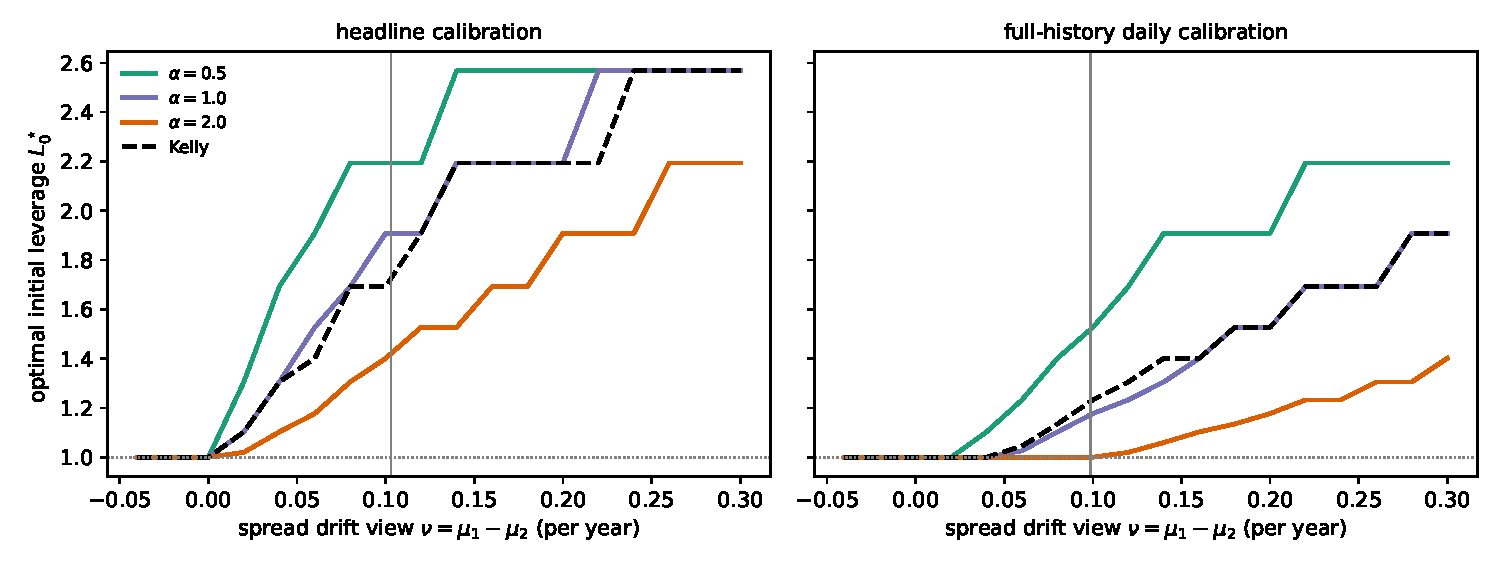
\includegraphics[width=\linewidth]{fig_buffer_drift.pdf}
    \end{column}
  \end{columns}
\end{frame}

% ------------------------------------------------------------
\begin{frame}{Can the Data Tell?}
  \small
  \[
    \operatorname{sd}(\widehat\mu)=\frac{\sigma}{\sqrt{\mathcal T}}\qquad\text{(calendar length only)}
  \]
  \begin{itemize}
    \item Sample spread drift $\hat\nu=+0.10$; s.e.\ $0.34$ (headline), $0.19$ (3.7 years)
    \item Separating $+0.10$ from $+0.05$ at 2 s.e.\ needs $\approx210$ years
    \item Posterior $\Pbb(\nu>\nu^\star)\approx$ \alert{one half} (carry-anchored prior); $\approx0.6$ (flat)
    \item Bayes--Kelly: lever iff $m>\nu^\star+\tfrac12Ts^2$ $\Rightarrow$ decided by the prior's shrinkage
    \item Reversed book (WETH collateral): $\nu=-0.11$ vs break-even $+0.10$ to $+0.19$
  \end{itemize}
  \vspace{0.4em}
  \alert{Optimal leverage hinges on an input the data cannot pin down}
\end{frame}

% ------------------------------------------------------------
\begin{frame}{Did Leverage Pay? Realised Replay of 37 Pairs}
  \scriptsize
  Hourly replay, Aave v3 2023-01 to 2026-10, protocol liquidation rules, no model
  \vspace{0.2em}

  \begin{columns}[T]
    \begin{column}{0.4\linewidth}
      \begin{tabular}{lcc}
      \toprule
      Roll & $L_0=1.25$ & $L_0=2$ \\
      \midrule
      1 day & $-0.04$ (4) & $-0.29$ (3) \\
      30 days & $-0.04$ (4) & $-0.33$ (4) \\
      Hold & $-0.02$ (12) & $-0.30$ (10) \\
      \bottomrule
      \end{tabular}
      \vspace{0.2em}

      Median excess log growth/yr (pairs where leverage paid)
      \vspace{0.3em}

      \begin{itemize}
        \item $1.25\times$ beat unlevered in \alert{4 of 37}, none significant
        \item 2025: $0/29$ cross-asset pair-years positive
        \item One cycle; BTC $\times3.6$, BTC/ETH $\times2.3$
      \end{itemize}
    \end{column}
    \begin{column}{0.58\linewidth}
      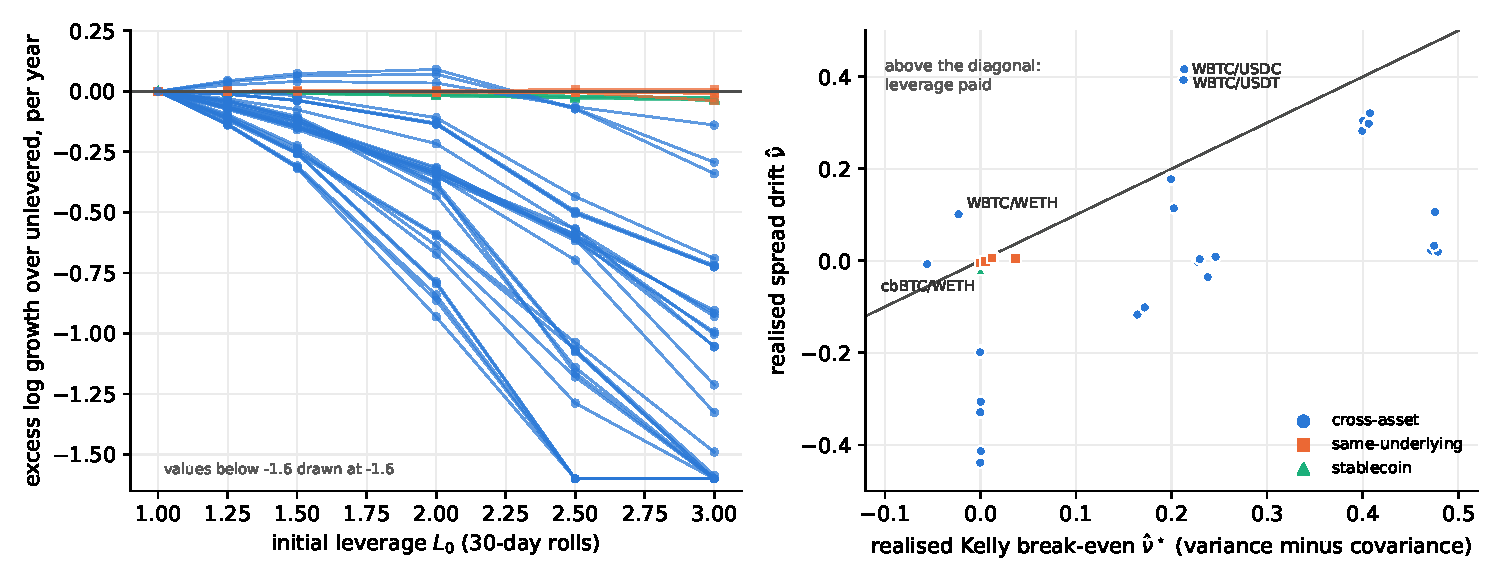
\includegraphics[width=\linewidth]{fig_realised_backtest.pdf}
    \end{column}
  \end{columns}
\end{frame}

% ------------------------------------------------------------
\begin{frame}{What the Replay Says About the Model}
  \small
  WBTC/WETH, annualised
  \vspace{0.2em}

  \begin{center}
  \begin{tabular}{lcc}
  \toprule
  & Model (independent jumps) & Realised, daily \\
  \midrule
  Correlation & $0.50$ & $0.81$ \\
  Covariance & $0.11$ & $0.24$ \\
  Spread variance & $0.23$ & $0.14$ \\
  Break-even $\nu^\star=\mathrm{Var}_1-\mathrm{Cov}$ & $+0.048$ & $-0.023$ \\
  \bottomrule
  \end{tabular}
  \end{center}
  \begin{itemize}
    \item $85\%$ of large days move both legs the same way: \alert{common jumps}
    \item Independent jumps cannot carry co-movement $\Rightarrow$ spread variance overstated by $60\%$
    \item Explains the out-of-sample over-prediction of $\liq$ ($1.3$--$1.6\times$)
    \item Fix: a common Poisson component (stays in the exponential-phase class)
  \end{itemize}
\end{frame}

% ------------------------------------------------------------
\begin{frame}{Interest-Rate Carry and Regimes}
  \small
  \begin{itemize}
    \item Deterministic carry $=$ per-leg drift shift $\mu_1\mapsto\mu_1+r_s$, $\mu_2\mapsto\mu_2+r_b$
    \item 37-pair pre-registered cross-section: carry worth $\le0.035$ barrier s.d.\ per month for cross-asset pairs
    \item Rate-curve kink $\Rightarrow$ two-state regime, $6\times6$ resolvent
    \item Calibrated: opening regime moves survival by $\le0.09$ pp at a month --- inert
    \item Depeg $d$ $=$ same book at $h_0+\log(1-d)$: low-volatility pairs are depeg-fragile
  \end{itemize}
\end{frame}

% ------------------------------------------------------------
\begin{frame}{Conclusions}
  \begin{itemize}
    \item Leveraged DeFi long--short $\rightarrow$ one scalar first-passage problem in $h_0$
    \item Killed moments, survival, exact recovery, overshoot law, bad debt, $\E\log W$: one $3\times3$ system
    \item Validated; three orders of magnitude faster than simulation
    \item Sizing: any objective hinges on a small break-even drift the data cannot estimate
    \item Ex post, leverage rarely paid (4/37 pairs at $1.25\times$, none significant)
    \item \alert{Output is the map, not a leverage number}
  \end{itemize}
  \vspace{0.6em}
  \textbf{Next}
  \begin{itemize}
    \item Common jump component
    \item Decision-theoretic sizing under drift uncertainty
    \item Endogenous utilization; dynamic collateral management
  \end{itemize}
  \vfill
  \begin{center}
    \large Thank you
  \end{center}
\end{frame}

% ------------------------------------------------------------
\begin{frame}{References}
  \footnotesize
  \bibliographystyle{abbrvnat}
  \bibliography{finance,additions}
\end{frame}

\end{document}
